\documentclass[12pt]{beamer}
\usepackage[portuguese]{babel}
\usepackage{anyfontsize}
\usepackage[all]{xy} 
\usepackage{MnSymbol,extarrows, tikz, pgfplots, graphicx, subfigure,float}
\usepackage{amsfonts,amsmath,amsthm,mathtools,mathrsfs}
\usepackage{ragged2e}
\usetheme{Berkeley}
\logo{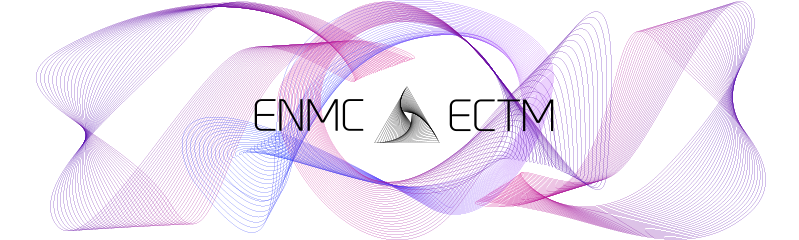
\includegraphics{logo.pdf}}
\graphicspath{ {/home/jefferson/Modelamento/} }
\title{Modelo de balan\c co energ\'etico hibr\'ido, contendo fontes intermitentes, baseada em  Programa\c{c}\~{a}o Din\^{a}mica Dual Estoc\'{a}stica}
\author{Jefferson Bezerra dos Santos}
\institute{Universidade Federal da Para\'iba }

\begin{document}
\begin{frame}
\titlepage % Print the title page as the first slide
\end{frame}

\begin{frame}{Sum\'ario}
\tableofcontents
\end{frame}

\section{Contextualiza\c c\~ao}
\begin{frame}{Contextualiza\c c\~ao}
Come\c cando	
\end{frame}

\section{Objetivos}
\begin{frame}{Objetivos}
\subsection{Objetivos Gerais}
Os objetivos gerais deste trabalho s\~ao:
\begin{itemize}
	\item An\'alise da varia\c c\~ao da produtibilidade de um modelo hidrot\'ermico em rela\c c\~ao aos cen\'arios de
		planejamento. 
	\item O modelamento misto de um modelo hidrot\'ermico em regime de complementaridade com fontes de energia renov\'aveis \'eolica e solar.
	\item An\'alise do custo esperado do sistema misto para verifica\c c\~ao de sua viabilidade.
	\item An\'alise dos principais cen\'arios que envolvem o sistema brasileiro. 
	\item Verificar se o modelo misto representa de maneira adequada o problema de planejamento energ\'etico.
\end{itemize}
\end{frame}

\begin{frame}
	\begin{justify}	
	\subsection{Objetivos Espec\'ificos}
	Os objetivos espec\'ificos deste trabalho s\~ao:
	\begin{itemize}
		\item Constru\c c\~ao de um algoritmo \'otimo  computacionalmente para o planejamento. 
		\item An\'alise de poss\'iveis erros do modelo.
	\end{itemize}
	\end{justify}
\end{frame}

\section{Metodologia}
\begin{frame}{Metodologia}
	\begin{justify}	
		Primeiramente realizou-se uma revis\~ao bibliogr\'afica sobre o setor energ\'etico brasileiro. Dessa revis\~ao
		observou-se que o Brasil \'e constitu\'ido por um sistema energ\'etico do tipo hidrot\'ermico de grande porte. No qual a
		principal metodologia utilizada \'e t\'ecnica de Programa\c c\~ao Din\^amica Dual Estoc\'astica, pois, tal t\'ecnica
		posssui a capacidade de realizar o planejamento sobre cen\'arios de incerteza. Al\'em, de possui uma implementa\c c\~ao
		computacional relativamente simples.
	\end{justify}
\end{frame}

\begin{frame}
	\begin{justify}	
	A segunda etapa do trabalho foi o entendimento da t\'ecnica e sua reprodu\c c\~ao computacional para teste de verifica\c
	c\~ao se tal t\'ecnica, realmente poderia ser utilizada como as pesquisas afirmavam. Foi verificado que realmente a
	t\'ecnica de Programa\c c\~ao Din\^amica Dual Estoc\'astica possui bons resultados e possui uma flexibilidade no
	planejamento de cen\'arios. 
	\end{justify}
\end{frame}

\begin{frame}
	\begin{justify}	
	Na terceira etapa buscou-se alguma melhoria ou resultado vantajoso do modelo que ainda n\~ao fosse  observado na base
	bibliogr\'afica. Dessa forma, os principais conceitos analizados foram: os cen\'arios, o custo esperado e a
	produtibilidade. Notou-se que uma varia\c c\~ao de produtibilidade fazia que o modelo modifica-se sua configura\c c\~ao
	de forma excepcional. Portanto, foram feitas extensivas simula\c c\~oes para averiguar se tal mudan\c ca realmente
	estava ocorrendo em todos os cen\'arios de planejamento  utilizados. Finalmente, constatou-se que realmente a mudan\c ca
	de produtibilidade fazia que o sistema modifica-se totalmente a sua configura\c c\~ao independentemente da probabilidade
	de ocorr\^encia do cen\'ario.
	\end{justify}
\end{frame}

\section{Despacho de energia}
\begin{frame}{Despacho de energia}
	\begin{justify}	
	No gerenciamento e transmiss\~ao da energia el\'etrica, o Brasil possui o Sistema Interligado Nacional
	(SIN) gerenciado pelo Operador Nacional de Energia (ONS) correspondendo as regi\~oes Sul, Sudeste,
	Centro-Oeste, Nordeste e parte do Norte. O SIN \'e respons\'avel por abrigar cerca de
	$96,6\%$ de toda a capacidade de produ\c c\~ao de energia do Brasil, seja por meio de fontes internas de energia
	ou pela importa\c c\~ao de energia como ocorre na usina de Itaipu mediante o controle compartilhado com o
	Paraguai. A ado\c c\~ao do SIN \'e justificada tendo por base: o interc\^ambio energ\'etico, a
	complementaridade entre fontes de gera\c c\~ao de energia e pela sua capacidade de expans\~ao.
	\end{justify}
\end{frame}

\begin{frame}
	\begin{justify}	
		No planejamento do sistema hidrot\'ermico brasileiro as caracter\'isticas que devem ser consideradas s\~ao:
		\begin{itemize}
		\item \textit{Sazonalidade intra natural}. Al\'em da variabilidade natural ocorre um varia\c c\~ao entre as esta\c
			c\~oes do ano. 
		\item \textit{A complementariedade e diversidade regional}. As bacias brasileiras possuem caracter\'isticas
			f\'isicas e clim\'aticas distintas. 
		\item \textit{O acoplamento espacial}. Na estrutura de cascata as usinas que est\~ao mais perto da jusante possuem depend\^encia
			de usinas mais perto da montante.
		\end{itemize}
	\end{justify}
\end{frame}

\begin{frame}
	\begin{justify}	
		\begin{itemize}
		\item \textit{O acoplamento temporal}. Na estrutura de cascata decis\~oes sobre a utiliza\c c\~ao possuem
			consequ\^encias no futuro. 
		\item \textit{Custo term\'eletrico}. Usinas term\'eletricas possuem um custo alto de produ\c c\~ao el\'etrica em
			rela\c c\~ao as hidrel\'etricas.
		\item \textit{Aspecto ambiental}. Usinas termel\'etricas possuem um alto impacto ambiental ocasionado pela queima de
			combust\'ivel.
	\end{itemize}
	\end{justify}
\end{frame}

\begin{frame}{Usinas em cascata}
	\begin{justify}	
		\begin{figure}[!htpb]
			\centering
			\resizebox{1.0\textwidth}{!}{%
			\input{material/cascataj.tex}}
			\label{st}
		\end{figure}
	\end{justify}
\end{frame}

\begin{frame}{Dilema do operador}
	\begin{justify}	
	 \begin{figure}[!h]
		 \centering
		 \resizebox{1.0\textwidth}{!}{%
		  \xymatrix@=1.0em{
			& & *+[F]{\text{CHUVA}} \ar[r]& *+[F]{\text{DECIS\~AO CORRETA}}\\
			& *+[F]{\text {USAR \ RESERVAT\'ORIO}} \ar[ur] \ar[dr] & &\\
			& & *+[F]{\text{SECA}} \ar[r] & *+[F]{\text{PREJU\'IZO}} \\
			*+ [F]{\text {OPERADOR}} \ar[uur] \ar[ddr] & & & \\
			& & *+[F]{ \text {CHUVA}} \ar[r] & *+ [F]{\text{PREJU\'IZO}}\\
			& *+ [F]{\text {USAR TERMEL\'ETRICA}} \ar[ur] \ar[dr]& &\\
			& & *+[F] {\text {SECA}} \ar[r] & *+[F]{\text{DECIS\~AO CORRETA}}
		 }}
	 \end{figure}
	\end{justify}
\end{frame}

\begin{frame}{Problema de 2 est\'agios}
	\begin{justify}	
	\begin{figure}[!h]
	 \centering
	 \resizebox{1.0\textwidth}{!}{%
	  \xymatrix@=1.0em{
		  & & *+[F]{\text{PLANEJAMENTO}}\ar[d]&\\ 
		  & & *+[F]{\text{CONFIGURA\c C\~AO INICIAL}} \ar[d]&\\  
		  & & *+[F]{\text{1 EST\'AGIO}} \ar[r] \ar[d]& *+[F]{\text{DECIS\~AO VI\'AVEL}} \ar[dd]\\
		  & & *+[F]{\text{CUSTO}} &\\   
		  & & & *+[F]{\text{2 EST\'AGIO}} \ar[d] \\ 
		  & & & *+[F]{\text{CUSTO}} 
	}}
	 \label{estagio}
	\end{figure}
	\end{justify}
\end{frame}

\begin{frame}{Modelo do despacho de energia}
	\begin{justify}	
	\begin{align}
		&\min \langle c_1,x_1\rangle + \langle c_2,x_2\rangle \nonumber \\
		&\mbox{tal que: }	A_1 x_1 \geq b_1 \nonumber \\
		&E_1 x_1 + A_2 x_2 \geq b_2 \nonumber
	\end{align}
	\begin{itemize}
	  \item $c_1$ e $c_2$ s\~ao vetores que representam os custos relacionados ao 1 e 2 est\'agio respectivamente;
	  \item $x_1$ e $x_2$ s\~ao vetores que representam as decis\~oes tomadas 1 e 2 est\'agios respectivamente;
	  \item $b_1$ e $b_2$ s\~ao os vetores de recursos no 1 e 2 est\'agios respectivamente;
	  \item $A_1$ e $A_2$ s\~ao matrizes que representam o acoplamento espacial;
	  \item $E_1$ \'e uma matriz que descreve o acoplamento temporal.
	\end{itemize}
	\end{justify}
\end{frame}

\begin{frame}{Programa\c c\~ao Din\^amica Dual Estoc\'astica}
	\begin{justify}	
		\begin{align*}
		{\text{min}} \ \ \langle c_1,x_1\rangle + p_1 {\beta}_{1} + p_2 {\beta}_{2} \\
		\textrm{Sujeito a:} \quad A_1 x_1 \geq b_1 \\
		{\pi}_{1}^{i}(b_{21} - E_1x_1) - {\beta}_{1} \leq 0 \\ 
		{\pi}_{2}^{j}(b_{22} - E_1x_1) - {\beta}_{2} \leq 0 \\ 
		i = 1, 2, \dots , P \\
		j = 1, 2, \dots , P. 
		\end{align*}
		\begin{itemize}
			\item $p_1$ e $p_2$ probabilidades associadas aos cen\'arios avaliados;
			\item $\beta_1$ e $\beta_2$ escalares derivados da transforma\c c\~ao dual;
			\item ${\pi}_{1}^{i}$ e ${\pi}_{2}^{i}$ v\'ertices do conjunto vi\'avel.
		\end{itemize}
	\end{justify}
\end{frame}

\begin{frame}{Mestre}
	\begin{justify}	
		\begin{align*}
		 \underset {s \backslash a}{\text{min}} \overbrace{\left < c_1,x_1\right >}^{\textrm{Primeiro estágio}} 
		 +\quad \underbrace {p_1 {\beta}_{1} + p_2 {\beta}_{2}}_{\textrm{Segundo estágio}}
		\end{align*}
		\text{Conjunto vi\'avel:}
		$\left \{ 
	 \begin{aligned}
		 A_1 x_1 \geq b_1 \\
		{\pi}_{1}^{i}(b_{21} - e_1x_1) - {\beta}_{1} \leq 0 \\ 
		{\pi}_{2}^{j}(b_{22} - e_1x_1) - {\beta}_{2} \leq 0 \\ 
		i = 1, 2, \dots , p \\
		j = 1, 2, \dots , p. 
	 \end{aligned}
	\right . 
	$
	\end{justify}
\end{frame}

\begin{frame}{Servos}
	\begin{align*}
		\txt{Servo 1:} \hspace{1cm}
	  \begin{split}	
		  \omega_1 = &\max \pi_1 (b_{21} - E_1x_1 ) \\
		&\mbox{tal que: }\pi_1 A_2  \leq c_2.
	  \end{split}
	\end{align*}

		\begin{align*}
			\txt{Servo 2:} \hspace{1cm}
	  \begin{split}	
		  \omega_2 = &\max \pi_2 (b_{22} - E_1x_1 ) \\
		&\mbox{tal que: }\pi_2 A_2  \leq c_2.
	  \end{split}
	\end{align*}
	\end{frame}

	\begin{frame}{Mestre completo}
	 \resizebox{1.2\textwidth}{!}{%
	  \xymatrix@C=0.1em{
		  &&*+[F]{\txt{Mestre completo \\ Resolver o problema encontrando $\beta_1$ e $\beta_2$.\\
		  \\ Verificar converg\^encia para \\ $|\beta_1 -
		  \omega_1|$ e $|\beta_2 - \omega_2| < $ toler\^ancia.}}\ar[dddl] \ar[dddr] 
		  & \hspace{2cm}\\ 
		  & & & & \\
		  & & & & \\
		  &*+[F]{\txt{SERVO 1\\ C\'alculo de $\omega_1$ \\$\omega_1 = \max \pi_1 (b_{21} - E_1x_1)$}}&
		  &*+[F]{\txt{SERVO 2 \\ C\'alculo de $\omega_2$ \\$\omega_2 = \max \pi_2 (b_{22} - E_1x_1 )$}}& & \hspace{2cm}
	}}
\end{frame}

\section{Resultados parciais}
\begin{frame}{Resultados parciais}
O sistema foi configurado de tal forma a garantir a demanda da regi\~ao dada por,
\begin{align*}
{\rho}_1*VTH1 + {\rho}_2*VTH2 + G1 + G2 = DEMANDA,
\end{align*}
onde:
\begin{itemize}
	\item $H_1$ e $H_2$ representam as hidrel\'etricas associadas ao sistema;
	\item $G_1$ e $G_2$ representam as termel\'etricas associadas ao sistema;
	\item $\rho_1$ e $\rho_2$ s\~ao os \'indices de produtibilidade das usinas H1 e H2;
	\item $VTH1$ e $VTH$  os volumes turbinados das hidrel\'etricas associadas.
\end{itemize}
\end{frame}
\begin{frame}{Balan\c co h\'idrico}
O sistema deve preservar o balan\c co hidr\'ico dada por,
{\setlength{\belowdisplayskip}{-4pt}
\begin{align*}
  \displaystyle Vt = VI + VIC - \left( VT + VV \right), 
\end{align*}}
onde : 
\begin{itemize}
	\item $V(t)$ representar o volume em qualquer instante de tempo;
	\item $VI$  volume inicial;
	\item $VIC$ volume incremental;
	\item $VV$ volume vertido.
\end{itemize}
\end{frame}
\begin{frame}{Gera\c c\~ao termel\'etrica}
\begin{justify}	
Por quest\~oes relacionadas ao custo e ao ambiente a gera\c c\~ao das termel\'etricas devem respeitar uma toler\^ancia de
gera\c c\~ao dada por:
\begin{align*}
	G_1 + G_2 \leq G_{max}
\end{align*}
\begin{itemize}
	\item $G_1$ gera\c c\~ao da termel\'etrica 1.
	\item $G_2$ gera\c c\~ao da termel\'etrica 2.
\end{itemize}
\end{justify}	
\end{frame}

\begin{frame}
\begin{figure}[!ht]
	\centering
		\includegraphics[width=6cm,height=6cm]{prob.0.1/simulacao.1.0/simula.pdf}
	\begin{center}	
		$\rho = 1.0$
	\end{center}
\end{figure}
\end{frame}

\section{Proposta da disserta\c c\~ao}

\begin{frame}
\end{frame}

\end{document}


